\chapter{Reference Measurements}

\section{Calibration Measurements in Neutron Reference Field}

Several ionization chambers have been calibrated at the National Metrology Institute of Germany (PTB). To carry out the calibration measurements on the chambers, a pure neutron field of quasi monoenergetic neutrons has been used to irradiate the chambers at different energies. Even though the source does not have the same energy configuration as the MEDAPP, it does generate fast neutrons at the same energy of the MEDAPP facilities. For this reason, the PTB facilities have been found to be suitable for the calibration of the devices. 

It is intended in this subsection to calculate the sensibility of the chamber. To calculate it for the PTW chambers TE-13 TM33053, TE-14 TM33053 and Mg-01 TM33054, respectively, the following formula is applied \cite{ReportPTW2018}:

\begin{align}
\label{eq:K_U,T}
    {k_{T,U} = \frac{k_a \: G_{aw} \: V_{LG} \: k_f \: Q}{KERMA}}
\end{align}

In Equation \ref{eq:K_U,T}, $k_a$ is the chamber specific air kerma calibration value, $G_{aw}$ is the $k_a$ effective dose conversion factor, $V_{LG}$ is the correction factor for the air-gas measurement, $k_f$ is the environmental correction factor for the pressure and temperature of the air and $Q$ is the accumulated charge in the ionization chamber. The constants used in Equation \ref{eq:K_U,T} are in Table \ref{tab:constants for PTB}. The environmental correction factor $k_f$ has been calculated using Equation \ref{eq:k_f}:

\begin{align}
\label{eq:k_f}
    {k_f = \frac{P_0 \: T}{P \: T_0}}
\end{align}

where $P_0$ and $T_0$ are reference pressure and temperature values. The  constant values are specific for each chamber type. A summary of the values used in the calculations is to be found in Table \ref{tab:constants for PTB}.

The temperature and atmospheric pressure have been measured for every measurement of the charge.
The value of ${KERMA}$ is the dose absorbed by the chamber and it has been measured to be between 5.4 and 5.6 \unit{\milli\gray}, depending on the device.
To take the measurements, each device has been positioned at the center of a platform as shown in Figure \ref{fig:Actual IC at PTW} and it has been irradiated by the neutron source perpendicularly.
\clearpage
\begin{table}[!h]
\centering
\begin{tabular}{llllllll}
                                              &  &  &  &  &  &                            &  \\
\cellcolor[HTML]{D9D9D9}P_0 {[}\unit{\milli\bar}{]}         &  &  &  &  &  & 1013.25                    &  \\
\cellcolor[HTML]{D9D9D9}T_0 {[}\unit{\kelvin}{}{]}            &  &  &  &  &  & 293.2                      &  \\
\cellcolor[HTML]{D9D9D9}G_{aw}                   &  &  &  &  &  & 1.112                      &  \\
\cellcolor[HTML]{D9D9D9}V_{LG} ($TE-13/14$)              &  &  &  &  &  & 0.861                      &  \\
\cellcolor[HTML]{D9D9D9}K_a  ($TE-13$) {[}\unit{\gray\per\coulomb}{]}  &  &  &  &  &  & $3.10 \cdot 10^{7}$ &  \\
\cellcolor[HTML]{D9D9D9}K_a  ($TE-14$){[}\unit{\gray\per\coulomb}{]}  &  &  &  &  &  & $3.09 \cdot 10^{7}$ &  \\
\cellcolor[HTML]{D9D9D9}V_{LG} ($Mg-01$)           &  &  &  &  &  & 0.688                      &  \\
\cellcolor[HTML]{D9D9D9}K_a ($Mg-01$){[}\unit{\gray\per\coulomb}{]}  &  &  &  &  &  & $2.68 \cdot 10^{7}$ &  \\
                                              &  &  &  &  &  &                            & 
\end{tabular}
\caption{Constants used in Equation \ref{eq:K_U,T}.}
\label{tab:constants for PTB}
\end{table}



\begin{figure}[!h]
\centering
\begin{minipage}{0.7\textwidth}
    \centering
    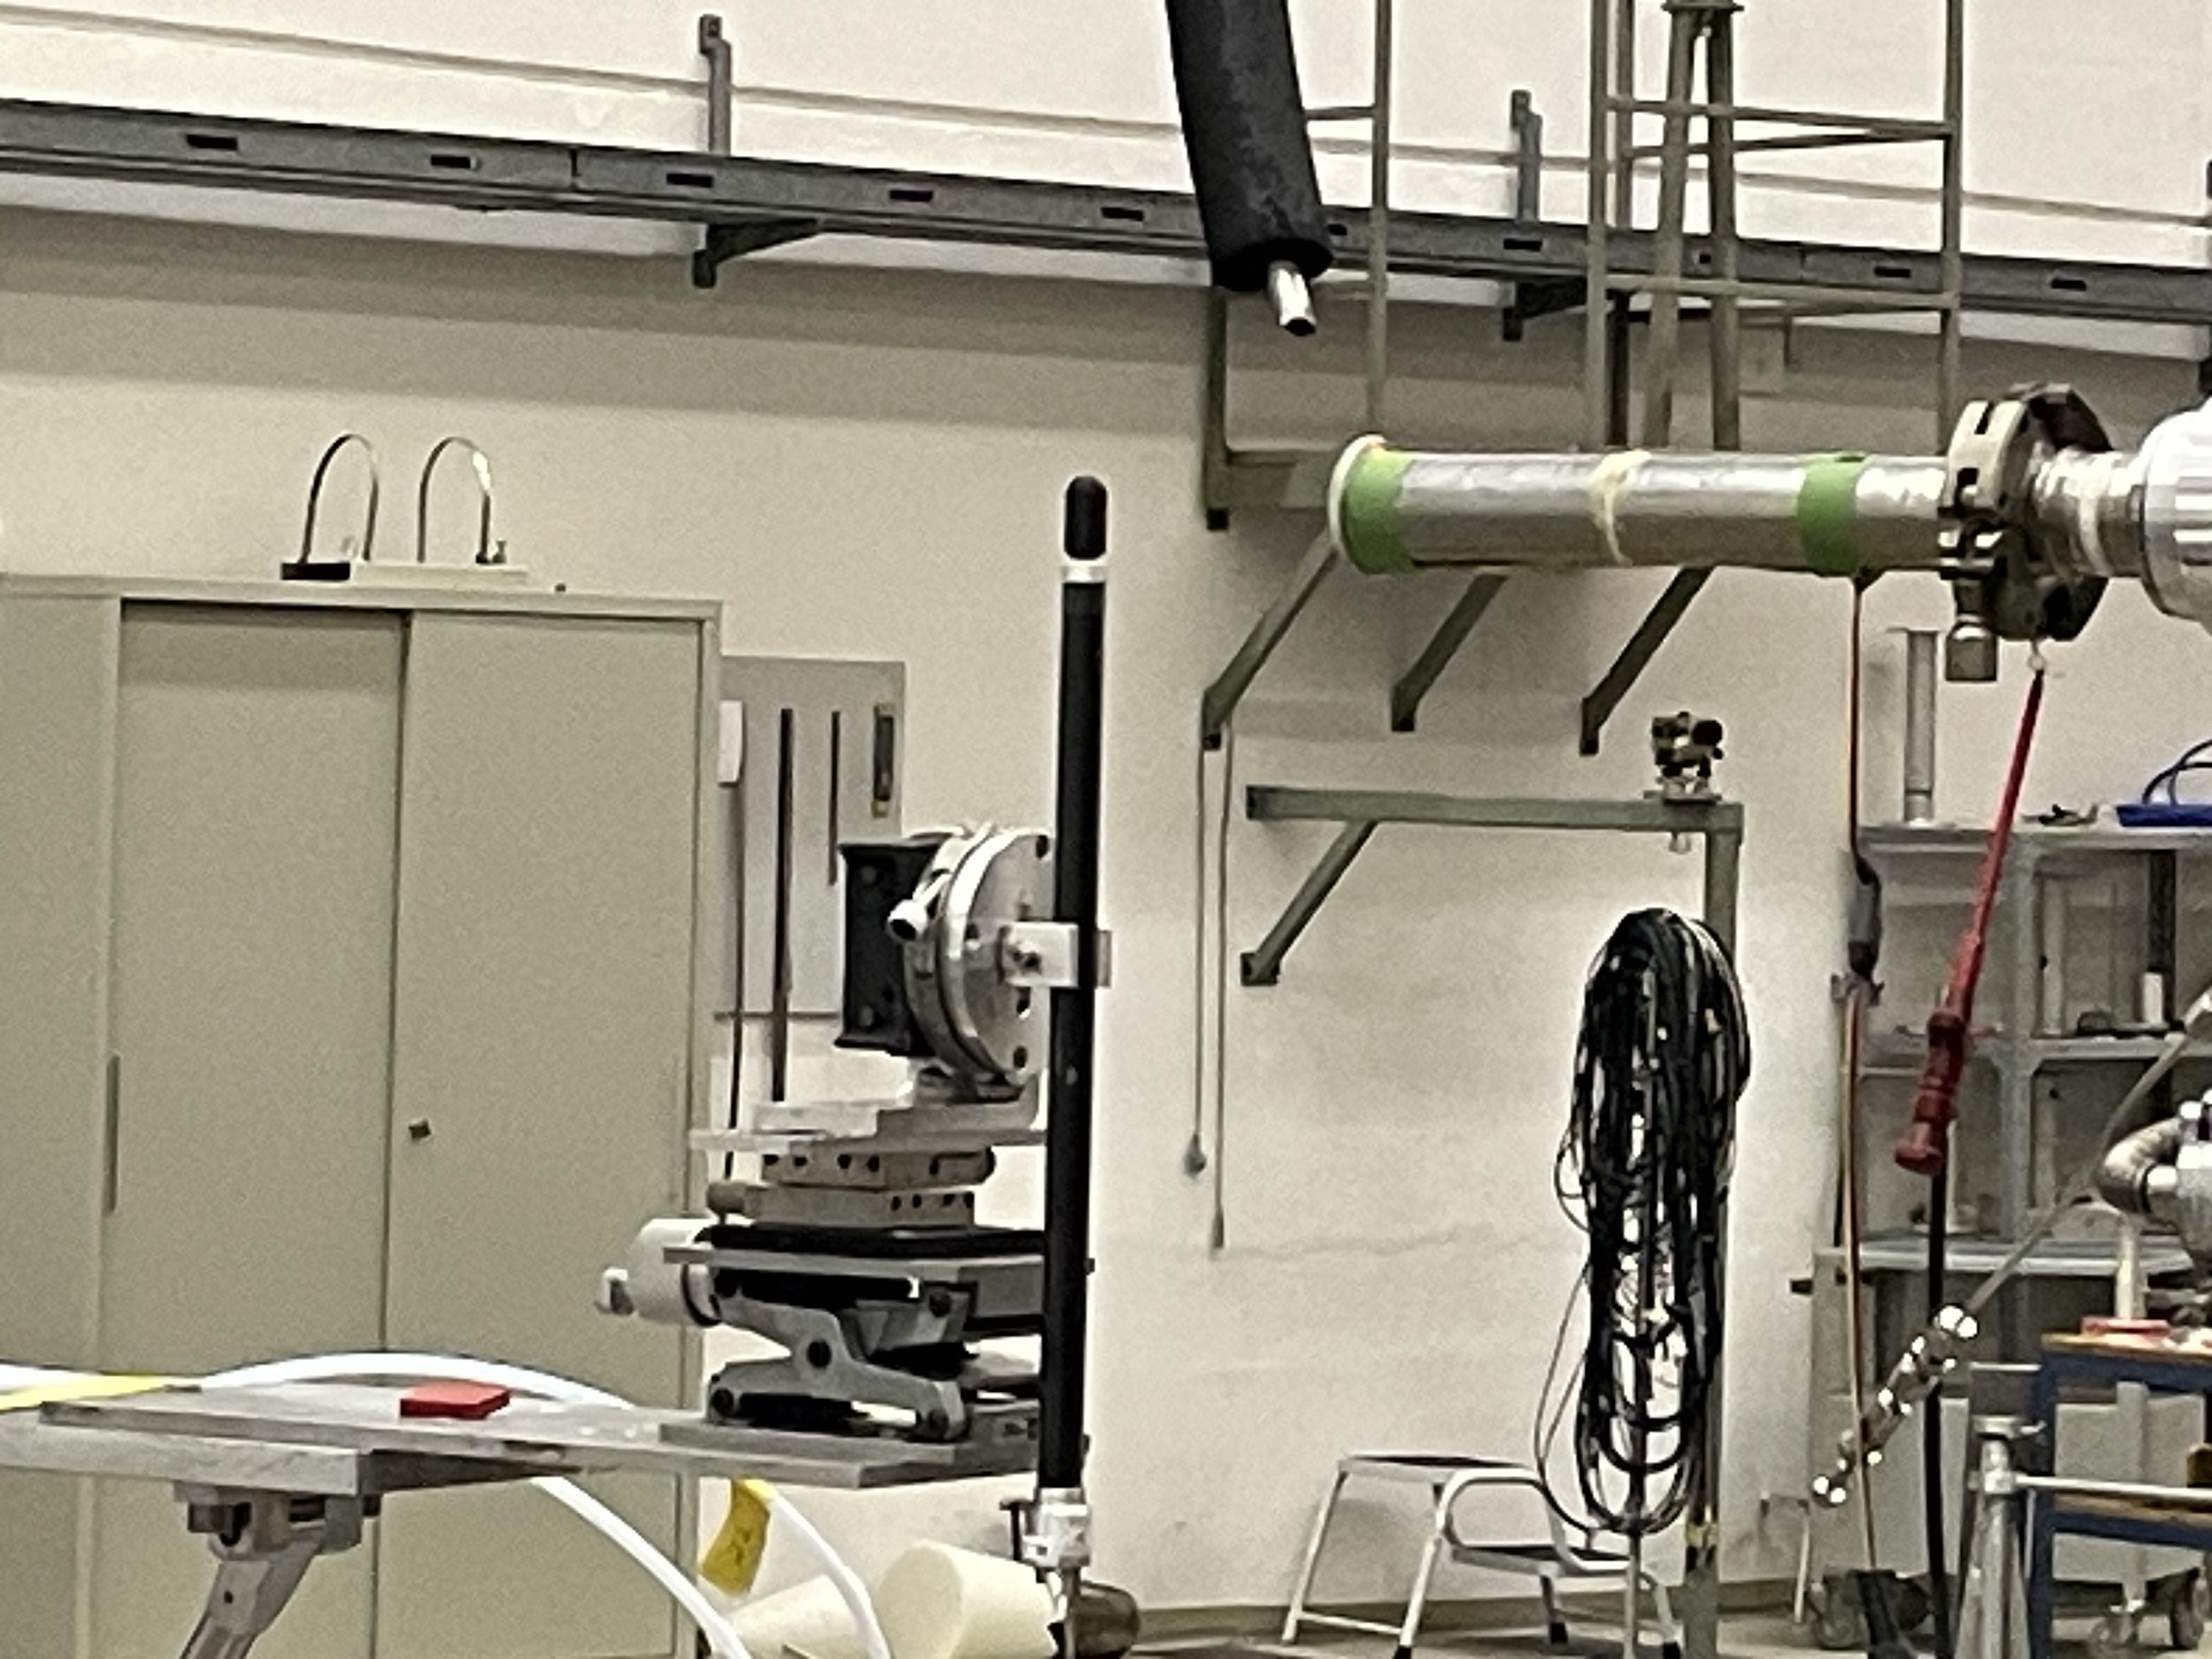
\includegraphics[width=\linewidth]{Master Thesis Manuel Galdon/figures/Build-up effect/PTW.jpeg} 
    \caption{Picture of a ionization chamber set up at PTB Braunschweig. The chamber is located in the middle and set up vertically. On the right side, the radiation source is pointing perpendicularly to the tip of the chamber.}
    \label{fig:Actual IC at PTW}
\end{minipage}
\end{figure}

The temperature and atmospheric pressure have been measured once for each energy. The values are in the range of 20.07 and 21.7 \unit{\celsius}, and 996.9 and 1001.9 \unit{\milli\bar}. The correction factor associated to this parameters, $k_f$, is around 1.01.
For the energies 1.2 and 2.5 \unit{\mega\electronvolt}, the kerma values, $k_{T,U}$ of each chamber have been calculated. The calculated $k_T$ and $k_U$ for the PTW chambers is:
%1.2 MeV
\begin{table}[!h]
\centering
\begin{tabular}{ccccc}
\hline
\rowcolor[HTML]{FCE0A7} 
\multicolumn{1}{|c}{\cellcolor[HTML]{FCE0A7}}                       & \multicolumn{4}{c|}{\cellcolor[HTML]{FCE0A7}1.2 \unit{\mega\electronvolt}}                                                                                                                  \\ \hline
                                                                    &                                 &                                         &                                         &                                                 \\ \cline{2-5} 
\multicolumn{1}{c|}{}                                               & \cellcolor[HTML]{D9D9D9}Chamber & \cellcolor[HTML]{D9D9D9}Charge {[}\unit{\pico\coulomb}{]} & \cellcolor[HTML]{D9D9D9}KERMA {[}\unit{\milli\gray}{]} & \multicolumn{1}{c|}{\cellcolor[HTML]{D9D9D9}k_T} \\ \cline{2-5} 
                                                                    &                                 &                                         &                                         &                                                 \\ \hline
\multicolumn{1}{|c|}{\cellcolor[HTML]{FEEFD1}}                      &                                 & 173.60                                  & 5.6                                     & \multicolumn{1}{c|}{0.932 \pm \:0.001}                      \\
\multicolumn{1}{|c|}{\cellcolor[HTML]{FEEFD1}}                      &                                 & 176.80                                  & 5.6                                     & \multicolumn{1}{c|}{0.950 \pm \:0.001}                      \\
\multicolumn{1}{|c|}{\cellcolor[HTML]{FEEFD1}}                      & \multirow{-3}{*}{TE-14}         & 177.40                                  & 5.6                                     & \multicolumn{1}{c|}{0.953 \pm \:0.001}                      \\ \cline{2-5} 
\multicolumn{1}{|c|}{\cellcolor[HTML]{FEEFD1}}                      &                                 &                                         &                                         &                                                 \\ \cline{2-5} 
\multicolumn{1}{|c|}{\cellcolor[HTML]{FEEFD1}}                      &                                 & 183.80                                  & 5.6                                     & \multicolumn{1}{c|}{0.984 \pm \:0.001}                      \\
\multicolumn{1}{|c|}{\cellcolor[HTML]{FEEFD1}}                      &                                 & 183.30                                  & 5.6                                     & \multicolumn{1}{c|}{0.982 \pm \:0.001}                      \\
\multicolumn{1}{|c|}{\multirow{-7}{*}{\cellcolor[HTML]{FEEFD1}PTW}} & \multirow{-3}{*}{TE-13}         & 183.20                                  & 5.6                                     & \multicolumn{1}{c|}{0.981 \pm \:0.001}                      \\ \hline
\end{tabular}

\end{table}

\begin{table}[!h]
\centering
\begin{tabular}{ccccc}
\cline{2-5}
\multicolumn{1}{c|}{}                                               & \cellcolor[HTML]{D9D9D9}Chamber & \cellcolor[HTML]{D9D9D9}Charge {[}\unit{\pico\coulomb}{]} & \cellcolor[HTML]{D9D9D9}KERMA {[}\unit{\milli\gray}{]} & \multicolumn{1}{c|}{\cellcolor[HTML]{D9D9D9}k_U} \\ \cline{2-5} 
                                                                    &                                 &                                         &                                         &                                                 \\ \hline
\multicolumn{1}{|c|}{\cellcolor[HTML]{FEEFD1}}                      &                                 & 72.59                                   & 5.6                                     & \multicolumn{1}{c|}{0.269 \pm \:0.001}                      \\
\multicolumn{1}{|c|}{\cellcolor[HTML]{FEEFD1}}                      &                                 & 73.37                                   & 5.6                                     & \multicolumn{1}{c|}{0.272 \pm \:0.001}                      \\
\multicolumn{1}{|c|}{\multirow{-3}{*}{\cellcolor[HTML]{FEEFD1}PTW}} & \multirow{-3}{*}{Mg-01}         & 72.72                                   & 5.6                                     & \multicolumn{1}{c|}{0.269 \pm \:0.001}                      \\ \hline
\end{tabular}
\caption{Calculated $k_T$ and $k_U$ for the PTW tissue equivalent and magnesium chambers at 1.2 \unit{\mega\electronvolt}, respectively.}
\end{table}

\\\\
% 2-5 MeV
\begin{table}[!h]
\centering
\begin{tabular}{ccccc}
\hline
\rowcolor[HTML]{FCE0A7} 
\multicolumn{1}{|c}{\cellcolor[HTML]{FCE0A7}}                       & \multicolumn{4}{c|}{\cellcolor[HTML]{FCE0A7}2.5 \unit{\mega\electronvolt}}                                                                                                                  \\ \hline
                                                                    &                                 &                                         &                                         &                                                 \\ \cline{2-5} 
\multicolumn{1}{c|}{}                                               & \cellcolor[HTML]{D9D9D9}Chamber & \cellcolor[HTML]{D9D9D9}Charge {[}\unit{\pico\coulomb}{]} & \cellcolor[HTML]{D9D9D9}KERMA {[}\unit{\milli\gray}{]} & \multicolumn{1}{c|}{\cellcolor[HTML]{D9D9D9}k_T} \\ \cline{2-5} 
                                                                    &                                 &                                         &                                         &                                                 \\ \hline
\multicolumn{1}{|c|}{\cellcolor[HTML]{FEEFD1}}                      &                                 & 185.6                                  & 5.4                                     & \multicolumn{1}{c|}{1.029 \pm \:0.001}                      \\
\multicolumn{1}{|c|}{\cellcolor[HTML]{FEEFD1}}                      &                                 & 186.2                                  & 5.4                                     & \multicolumn{1}{c|}{1.033 \pm \:0.001}                      \\
\multicolumn{1}{|c|}{\cellcolor[HTML]{FEEFD1}}                      & \multirow{-3}{*}{TE-14}         & 186.1                                  & 5.4                                     & \multicolumn{1}{c|}{1.032 \pm \:0.001}                      \\ \cline{2-5} 
\multicolumn{1}{|c|}{\cellcolor[HTML]{FEEFD1}}                      &                                 &                                         &                                         &                                                 \\ \cline{2-5} 
\multicolumn{1}{|c|}{\cellcolor[HTML]{FEEFD1}}                      &                                 & 186.2                                  & 5.4                                     & \multicolumn{1}{c|}{1.038 \pm \:0.001}                      \\
\multicolumn{1}{|c|}{\cellcolor[HTML]{FEEFD1}}                      &                                 & 186.6                                  & 5.4                                     & \multicolumn{1}{c|}{1.040 \pm \:0.001}                      \\
\multicolumn{1}{|c|}{\multirow{-7}{*}{\cellcolor[HTML]{FEEFD1}PTW}} & \multirow{-3}{*}{TE-13}         & 186.1                                  & 5.6                                     & \multicolumn{1}{c|}{1.037 \pm \:0.001}                      \\ \hline
\end{tabular}

\end{table}
\\\\
\begin{table}[!h]
\centering
\begin{tabular}{ccccc}
\cline{2-5}
\multicolumn{1}{c|}{}                                               & \cellcolor[HTML]{D9D9D9}Chamber & \cellcolor[HTML]{D9D9D9}Charge {[}\unit{\pico\coulomb}{]} & \cellcolor[HTML]{D9D9D9}KERMA {[}\unit{\milli\gray}{]} & \multicolumn{1}{c|}{\cellcolor[HTML]{D9D9D9}k_U} \\ \cline{2-5} 
                                                                    &                                 &                                         &                                         &                                                 \\ \hline
\multicolumn{1}{|c|}{\cellcolor[HTML]{FEEFD1}}                      &                                 & 52.54                                   & 5.4                                     & \multicolumn{1}{c|}{0.202 \pm \:0.001}                      \\
\multicolumn{1}{|c|}{\cellcolor[HTML]{FEEFD1}}                      &                                 & 52.41                                   & 5.4                                     & \multicolumn{1}{c|}{0.202 \pm \:0.001}                      \\
\multicolumn{1}{|c|}{\multirow{-3}{*}{\cellcolor[HTML]{FEEFD1}PTW}} & \multirow{-3}{*}{Mg-01}         & 52.41                                   & 5.4                                     & \multicolumn{1}{c|}{0.202 \pm \:0.001}                      \\ \hline
\end{tabular}
\caption{Calculated $k_T$ and $k_U$ for the PTW tissue equivalent and magnesium chambers at 2.5 \unit{\mega\electronvolt}, respectively.}
\end{table}

\\\\ %5 MeV

%\clearpage
%In the measurements for the 5 \unit{\mega\electronvolt}, the value of KERMA could not be measured at PTW. Instead and for the purpose of this calculations, a value of 5 \unit{\milli\gray} has been selected. 

%\begin{table}[!h]
%\centering
%\begin{tabular}{ccccc}
%\hline
%\multicolumn{5}{|c|}{\cellcolor[HTML]{FCE0A7}5   \unit{\mega\electronvolt}}                                                                                                                                                                                       \\ \hline
%\multicolumn{1}{l}{}                                                & %\multicolumn{1}{l}{}            & \multicolumn{1}{l}{}                    & %\multicolumn{1}{l}{}                    & \multicolumn{1}{l}{}                            \\
%\multicolumn{1}{l}{}                                                & %\multicolumn{1}{l}{}            & \multicolumn{1}{l}{}                    & %\multicolumn{1}{l}{}                    & \multicolumn{1}{l}{}                         %   \\ \cline{2-5} 
%\multicolumn{1}{l|}{}                                               & \cellcolor[HTML]{D9D9D9}Chamber & \cellcolor[HTML]{D9D9D9}Charge {[}\unit{\pico\coulomb}{]} & \cellcolor[HTML]{D9D9D9}KERMA {[}\unit{\milli\gray}{]} & \multicolumn{1}{c|}{\cellcolor[HTML]{D9D9D9}k_T} \\ \cline{2-5} 
%\multicolumn{1}{l}{}                                                & \multicolumn{1}{l}{}            & \multicolumn{1}{l}{}                    & \multicolumn{1}{l}{}                    & \multicolumn{1}{l}{}                            \\ \hline
%\multicolumn{1}{|c|}{\cellcolor[HTML]{FEEFD1}}                      &                                 & 186.8                                 & 5                                       & \multicolumn{1}{c|}{1.126 \pm \:0.001}                      \\
%\multicolumn{1}{|c|}{\cellcolor[HTML]{FEEFD1}}                      &                                 & 186.7                                 & 5                                       & \multicolumn{1}{c|}{1.125 \pm \:0.001}                      \\
%\multicolumn{1}{|c|}{\cellcolor[HTML]{FEEFD1}}                      & \multirow{-3}{*}{TE-14}         & 185.6                                 & 5                                       & \multicolumn{1}{c|}{1.119 \pm \:0.001}                      \\ \cline{2-5} 
%\multicolumn{1}{|c|}{\cellcolor[HTML]{FEEFD1}}                      & \multicolumn{1}{l}{}            &                                         &                                         &                                                 \\ \cline{2-5} 
%\multicolumn{1}{|c|}{\cellcolor[HTML]{FEEFD1}}                      &                                 & 186.4                                 & 5                                       & \multicolumn{1}{c|}{1.126 \pm \:0.001}                      \\
%\multicolumn{1}{|c|}{\cellcolor[HTML]{FEEFD1}}                      &                                 & 187.7                                 & 5                                       & \multicolumn{1}{c|}{1.133 \pm \:0.001}                      \\
%\multicolumn{1}{|c|}{\multirow{-7}{*}{\cellcolor[HTML]{FEEFD1}PTW}} & \multirow{-3}{*}{TE-13}         & 188.3                                 & 5                                       & \multicolumn{1}{c|}{1.137 \pm \:0.001}                      \\ \hline
%\end{tabular}
%\end{table}

%\begin{table}
%\centering
%\begin{tabular}{cccccc}
%\multicolumn{1}{l}{}                                                & \multicolumn{1}{l}{}                                                         & \multicolumn{1}{l}{}            & \multicolumn{1}{l}{}                    & \multicolumn{1}{l}{}                    & \multicolumn{1}{l}{}                            \\
%\multicolumn{1}{l}{}                                                & \multicolumn{1}{l}{}                                                         & \multicolumn{1}{l}{}            & \multicolumn{1}{l}{}                    & \multicolumn{1}{l}{}                    & \multicolumn{1}{l}{}                            \\ \cline{3-6} 
%\multicolumn{1}{l}{}                                                & \multicolumn{1}{c|}{}                                                        & \cellcolor[HTML]{D9D9D9}Chamber & \cellcolor[HTML]{D9D9D9}Charge {[}\unit{\pico\coulomb}{]} & \cellcolor[HTML]{D9D9D9}KERMA {[}\unit{\milli\gray}{]} & \multicolumn{1}{c|}{\cellcolor[HTML]{D9D9D9}k_U} \\ \cline{3-6} 
%\multicolumn{1}{l}{}                                                & \multicolumn{1}{l}{}                                                         & \multicolumn{1}{l}{}            & \multicolumn{1}{l}{}                    & \multicolumn{1}{l}{}                    & \multicolumn{1}{l}{}                            \\ \hline
%\multicolumn{1}{|c}{\cellcolor[HTML]{FEEFD1}}                       & \multicolumn{1}{c|}{\cellcolor[HTML]{FEEFD1}}                                &                                 & 45.050                                  & 5                                       & \multicolumn{1}{c|}{0.188 \pm \:0.001}                      \\
%\multicolumn{1}{|c}{\cellcolor[HTML]{FEEFD1}}                       & \multicolumn{1}{c|}{\cellcolor[HTML]{FEEFD1}}                                &                                 & 45.810                                  & 5                                       & \multicolumn{1}{c|}{0.191 \pm \:0.001}                      \\
%\multicolumn{1}{|c}{\cellcolor[HTML]{FEEFD1}}                       & \multicolumn{1}{c|}{\multirow{-3}{*}{\cellcolor[HTML]{FEEFD1}1mm Mg cap}}    & \multirow{-3}{*}{Mg-01}         & 46.500                                  & 5                                       & \multicolumn{1}{c|}{0.194 \pm \:0.001}                      \\ \cline{3-6} 
%\multicolumn{1}{|c}{\cellcolor[HTML]{FEEFD1}}                       & \multicolumn{1}{l|}{\cellcolor[HTML]{FEEFD1}}                                & \multicolumn{1}{l}{}            &                                         &                                         &                                                 \\ \cline{3-6} 
%\multicolumn{1}{|c}{\cellcolor[HTML]{FEEFD1}}                       & \multicolumn{1}{c|}{\cellcolor[HTML]{FEEFD1}}                                &                                 & 45.840                                  & 5                                       & \multicolumn{1}{c|}{0.191 \pm \:0.001}                      \\
%\multicolumn{1}{|c}{\cellcolor[HTML]{FEEFD1}}                       & \multicolumn{1}{c|}{\cellcolor[HTML]{FEEFD1}}                                &                                 & 46.010                                  & 5                                       & \multicolumn{1}{c|}{0.192 \pm \:0.001}                      \\
%\multicolumn{1}{|c}{\cellcolor[HTML]{FEEFD1}}                       & \multicolumn{1}{c|}{\multirow{-3}{*}{\cellcolor[HTML]{FEEFD1}2   mm Mg cap}} & \multirow{-3}{*}{Mg-01}         & 44.690                                  & 5                                       & \multicolumn{1}{c|}{0.186 \pm \:0.001}                      \\ \cline{3-6} 
%\multicolumn{1}{|c}{\cellcolor[HTML]{FEEFD1}}                       & \multicolumn{1}{l|}{\cellcolor[HTML]{FEEFD1}}                                & \multicolumn{1}{l}{}            &                                         &                                         &                                                 \\ \cline{3-6} 
%\multicolumn{1}{|c}{\cellcolor[HTML]{FEEFD1}}                       & \multicolumn{1}{c|}{\cellcolor[HTML]{FEEFD1}}                                &                                 & 45.510                                  & 5                                       & \multicolumn{1}{c|}{0.189 \pm \:0.001}                      \\
%\multicolumn{1}{|c}{\cellcolor[HTML]{FEEFD1}}                       & \multicolumn{1}{c|}{\cellcolor[HTML]{FEEFD1}}                                &                                 & 44.660                                  & 5                                       & \multicolumn{1}{c|}{0.186 \pm \:0.001}                      \\
%\multicolumn{1}{|c}{\multirow{-11}{*}{\cellcolor[HTML]{FEEFD1}PTW}} & \multicolumn{1}{c|}{\multirow{-3}{*}{\cellcolor[HTML]{FEEFD1}No cap}}        & \multirow{-3}{*}{Mg-01}         & 44.990                                  & 5                                       & \multicolumn{1}{c|}{0.187 \pm \:0.001}                      \\ \hline
%\end{tabular}
%\end{table}
\clearpage

\subsection{Data Comparison}

The same measurements were performed by the MEDAPP team at the same facility for the same ionization chambers in 2018. According to the calibration performed by Dr. Markus Kellermeier and Dr. Lucas Sommer \cite{ReportPTW2018}, the values of the measured kerma have varied at 2.5 \unit{\mega\electronvolt} with regards to those stated on the report. 

A comparison of the values of the sensibility for the ionization chamber is presented. The values of $k_U$ and $k_T$ are calculated from the initial measurements of the charge and KERMA of the calibration of 2018 \cite{ReportPTW2018} and are plotted in the next figure:

\begin{figure}[!h]
\centering
\begin{minipage}{0.8\textwidth}
    \centering
    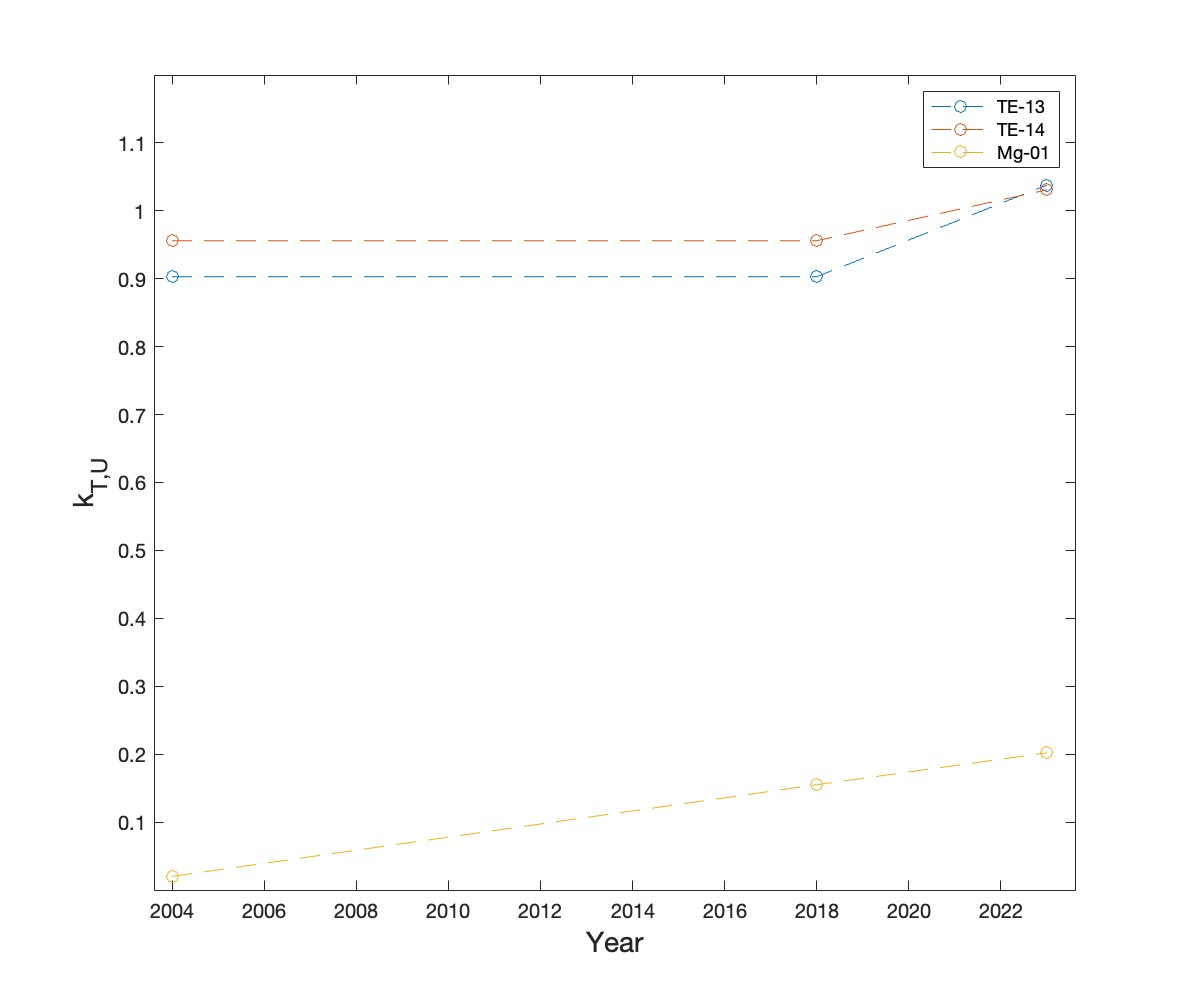
\includegraphics[width=\linewidth]{Master Thesis Manuel Galdon/figures/Build-up effect/Comparison k.jpg} 
    \caption{Values of $k_U$ and $k_T$ measured at PTB in different years for 2.5 \unit{\mega\electronvolt}.}
    \label{fig:Comparison of k at PTB}
\end{minipage}
\end{figure}

The sensibility in 2004 is taken from \textit{Bericht zur Basisdosimetrie für medizinische Bestrahlung an der Strahlkonverteranlage am FRM-II Garching (2006)} \cite{basisdosimetrieMEDAPP} as 0.943 for TE-13 and TE-14 and assumed to be unchanged in 2018. For Mg-01, the value in 2004 is 0.02 \cite{basisdosimetrieMEDAPP}. A linear fit is also performed from the data of the Figure \ref{fig:Comparison of k at PTB} in order to compare the slopes:
\newpage
\begin{table}[!h]
\centering
\begin{tabular}{|c|c|}
\hline
\rowcolor[HTML]{A9D9C6} 
Chamber & Slope [10^{-3}]\\ \hline
TE-13           & 5.6                                \\ \hline
TE-14           & 3.1                               \\ \hline
Mg-01           & 9.6                               \\ \hline
\end{tabular}
\caption{Slope comparison of the linear fit for the sensibility of the chambers TE-13, TE-14 and Mg-01 at 2.5 \unit{\mega\electronvolt}.}
\label{table: Slope comparison for MEDAPP source at the energy deposition. Neutrons}
\end{table}

In this comparison, TE-13 and TE-14 show similar and relatively higher slopes, between $3.1 \cdot 10^{-3}$ and $5.6 \cdot 10^{-3}$ [year]$^{-1}$, implying a consistent increase in sensibility over the measured period. On the other hand, Mg-01 has a lower slope of $9.6 \cdot 10^{-3}$ [year]$^{-1}$, indicating a less pronounced change in sensibility compared to the tissue equivalent chambers.

\section{Build-up Effect}
As neutrons slow down i.e. lose energy, the likelihood of interacting with atomic nuclei rises, resulting in a region near the material surface known as the "build-up region" of the material where neutron fluence increases significantly. In the next plot, that behaviour is clearly noticeable. In Figure \ref{fig:Cross seciton neutrons}, the cross section of neutrons is assessed on selected isotopes and hydrogen-rich plastic foils \cite{NeutronImaging}.

\begin{figure}[!h]
\centering
\begin{minipage}{0.9\textwidth}
    \centering
    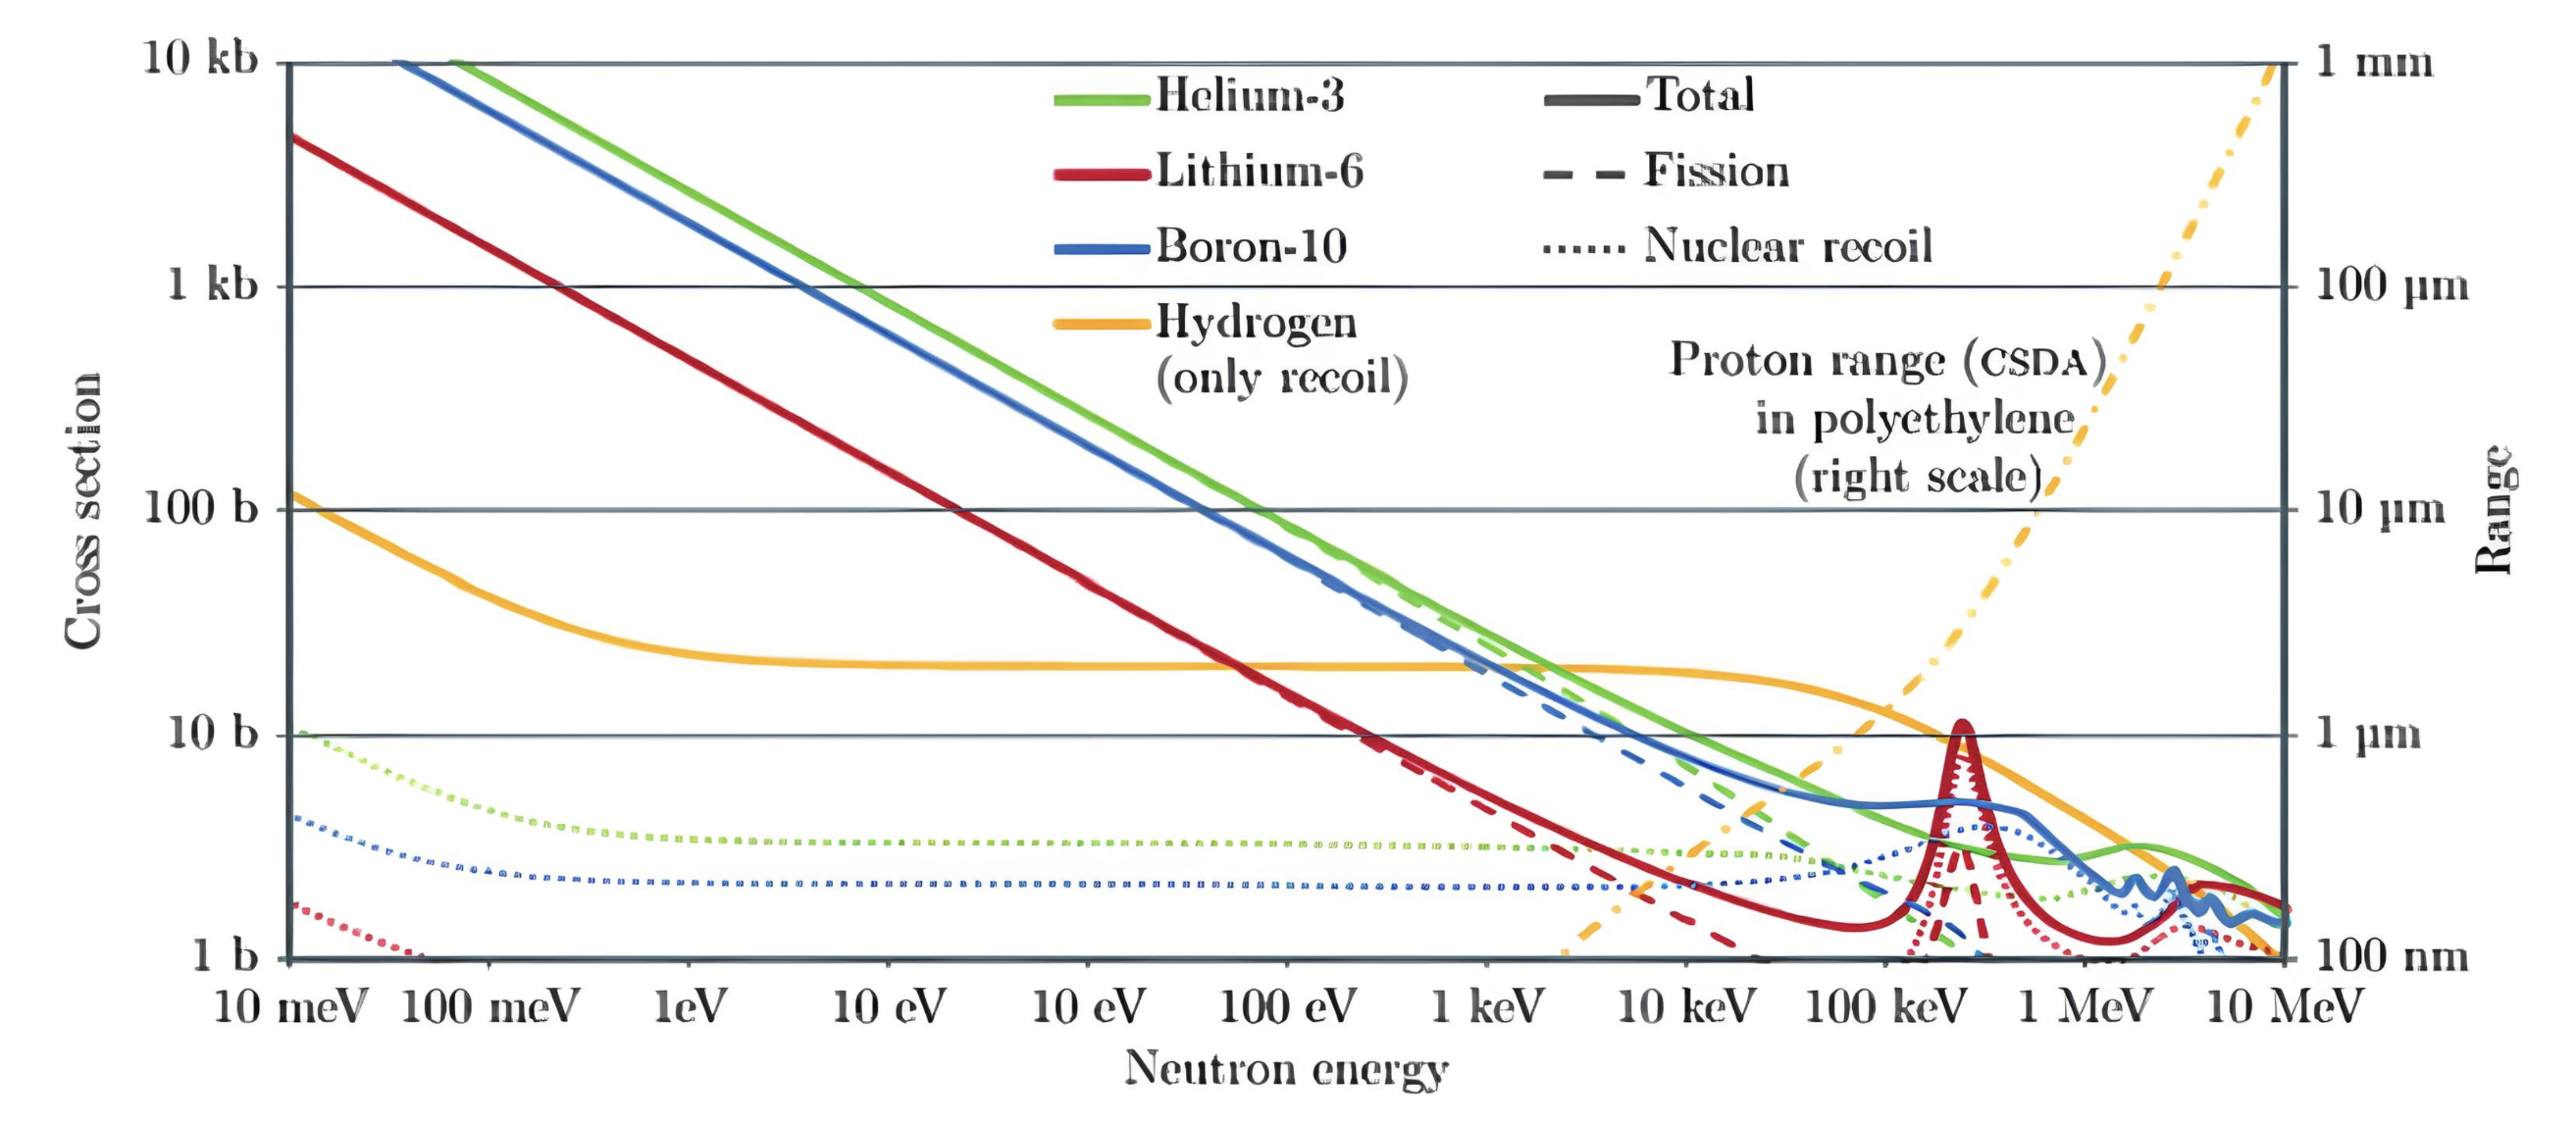
\includegraphics[width=\linewidth]{Master Thesis Manuel Galdon/figures/Build-up effect/cross section neutrons.png} 
    \caption{Cross section measured in  \textit{barns} of various selected isotopes as a function of neutron energy. }
    \label{fig:Cross seciton neutrons}
\end{minipage}
\end{figure}

There are definite regions in Figure \ref{fig:Cross seciton neutrons} where the cross section peaks at a certain value or experiments slight increase (depending on the target nuclei) to finally descend again at a higher neutron temperature. When this happens, the energy deposited in the material undergoes a fluctuation. This is the \textit{build-up effect} and it might take place in both magnesium and tissue equivalent plastic ionization chambers. In this section, the simulation of the effect in both materials is presented. In order to study it, the simulations are designed using a cylinder whose radius is 0.75 \unit{\milli\meter}, and the energy deposition per cubic centimeter at different energies is measured. Finally, the source used in the simulations is a monochromatic plane neutron, as it was used at PTB.
\subsection{Build-up Effect in Tissue Equivalent Plastic A-150 (TE)}
With a density of 1.27 \unit{\gram\per\cubic\centi\meter} according to the \textit{ESTAR Database} \cite{ESTAR}, the plastic shows a clear build-up effect that becomes more notable as the energy of the incoming beam rises. Using the \textbf{plane neutron source}, the tissue equivalent cylinder behaves as follows:

\begin{figure}[!h]
\centering
\begin{minipage}[t]{0.8\textwidth}
    \centering
    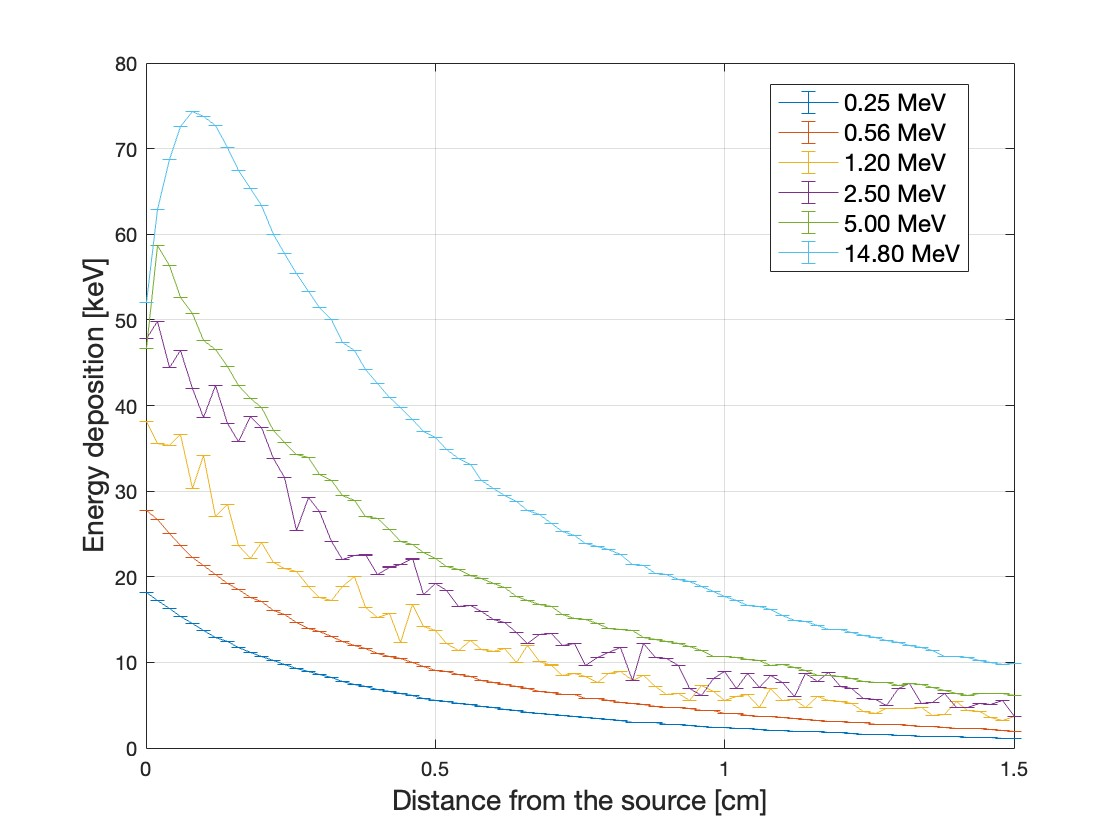
\includegraphics[width=\linewidth, height=9cm]{Master Thesis Manuel Galdon/figures/Build-up effect/TE cylinder with plane source.jpg} 
    \caption{Energy deposition plot of a TE cylinder plot using a plane neutron source at different energies. There is no gap between the source plane and the cylinder.}
    \label{fig:A150 cylinder with plane neutron source}
\end{minipage}
\end{figure}

Here, neutrons are primarily scattered by the constituent nuclei. As these neutrons travel deeper into the material, they engage in numerous interactions, transferring energy to atomic nuclei and generating secondary charged particles. This chain of interactions results in an increased dose deposition within the plastic at greater depths, which explains the slight displacement of the peak of energy deposition to the right as the energy of the beam increases, giving rise to the buildup effect that is observed beyond the energy of 2.5 \unit{\mega\electronvolt}.

\subsection{Build-up Effect in Magnesium}
In this simulation, the same configuration for the neutron source as in the case of the TE material is used. The deposited energy in the  magnesium cylinder is:

\begin{figure}[!h]
\centering
\begin{minipage}{0.8\textwidth}
    \centering
    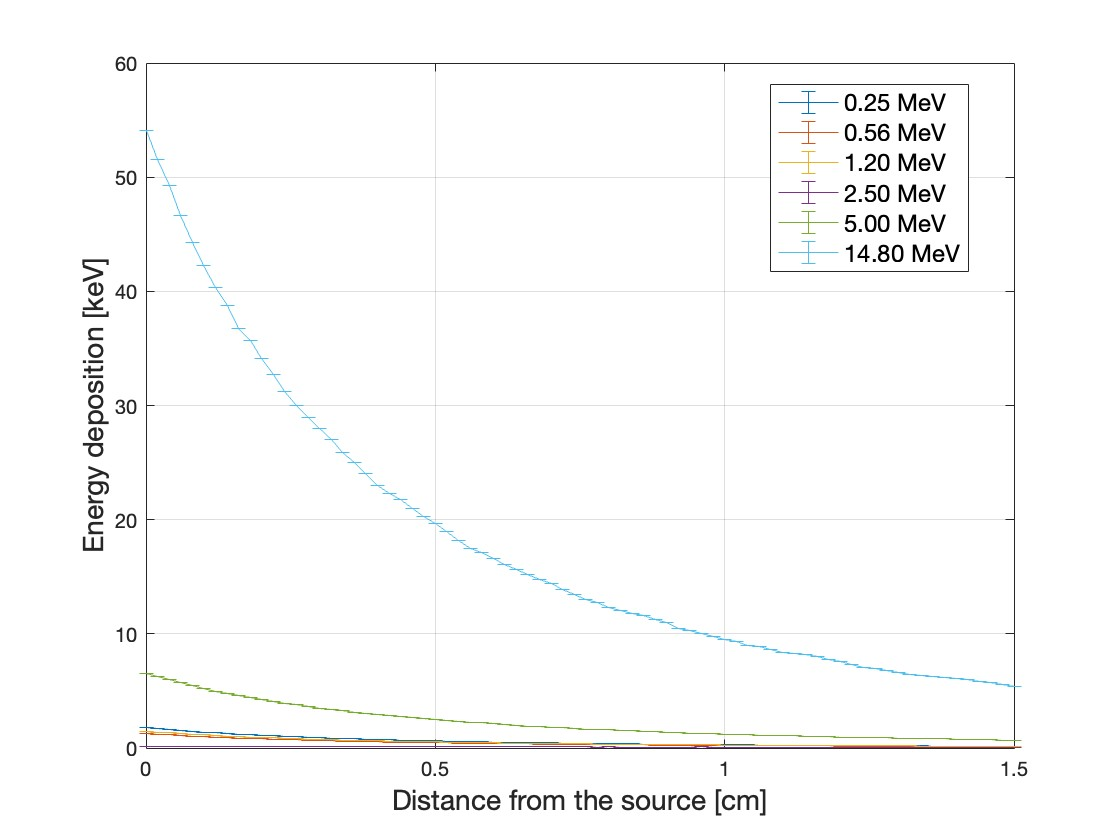
\includegraphics[width=\linewidth]{Master Thesis Manuel Galdon/figures/Build-up effect/Mg cylinder only.jpg}
    \label{fig:IC}
\end{minipage}
    \caption{Energy deposition plot of the magnesium cylinder plot using a plane neutron source at different energies. There is no gap between the source plane and the cylinder.}
    \label{fig:Mg cylinder with plane neutron source}
\end{figure}

According to the plot on Figure \ref{fig:Mg cylinder with plane neutron source}, there is apparently no build-up effect in this material. The difference between the energy deposition for the highest energy and the lower is too big to notice the response of the cylinder properly. For this reason, a close-up to the lowest energies is provided in the next plot: 
\newpage
\begin{figure}[!h]
\centering
\begin{minipage}{0.8\textwidth}
    %\renewcommand{\thefigure}{A} % Set the label of the first figure to A
    \centering
    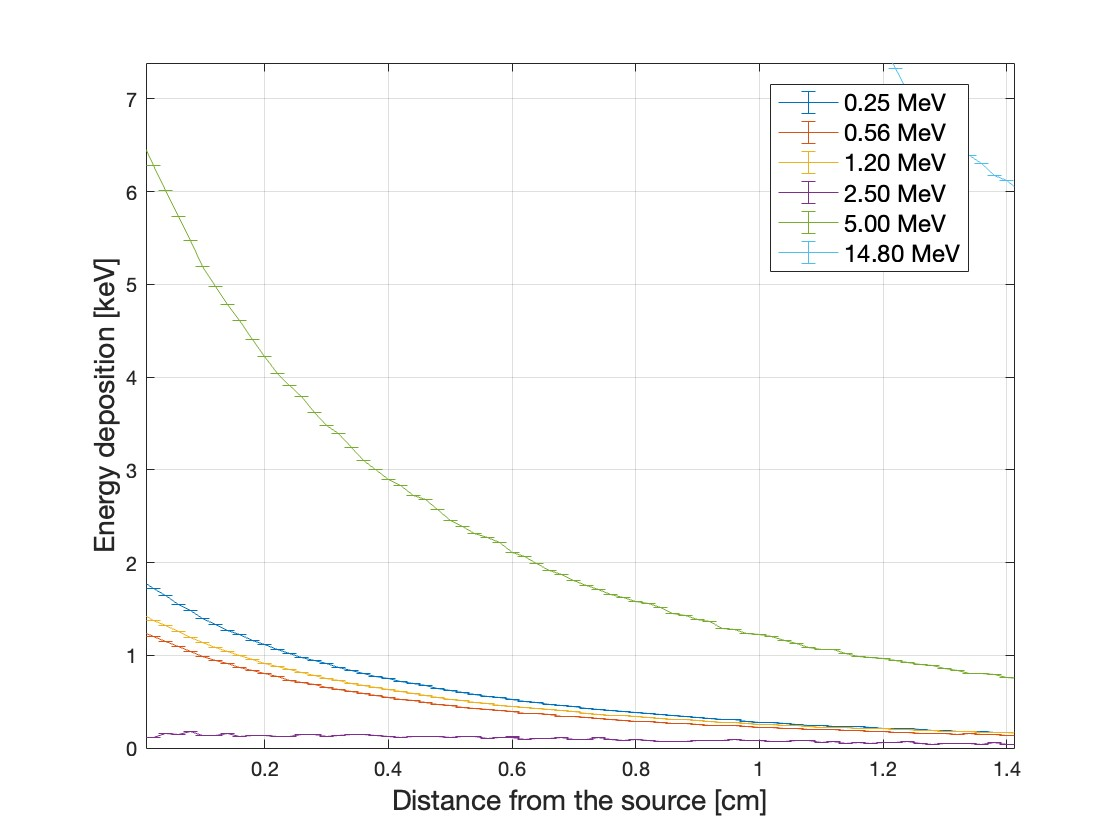
\includegraphics[width=\linewidth]{Master Thesis Manuel Galdon/figures/Build-up effect/Mg cylinder only - detail.jpg}
\end{minipage}
    \caption{Close-up of the energy deposition plot of the magnesium cylinder plot using a plane neutron source at different energies. There is no gap between the source plane and the cylinder.}
    \label{fig:Mg cylinder in detail with plane neutron source}
\end{figure}

The lines of the energies 0.25 and 2.5 \unit{\mega\electronvolt} appear to be switched, while the expected result should be a directly proportional relationship between the energy of the beam and the energy deposition.
This behaviour is due to the neutrons hitting the nuclei at a \textbf{resonance} energy for which the cross section of the atom grows significantly. In order to confirm that, the cross section of the magnesium against the energy of the incident neutron is plotted next:
\newpage
\begin{figure}[!h]
\centering
\begin{minipage}[t]{0.8\textwidth}
    \centering
    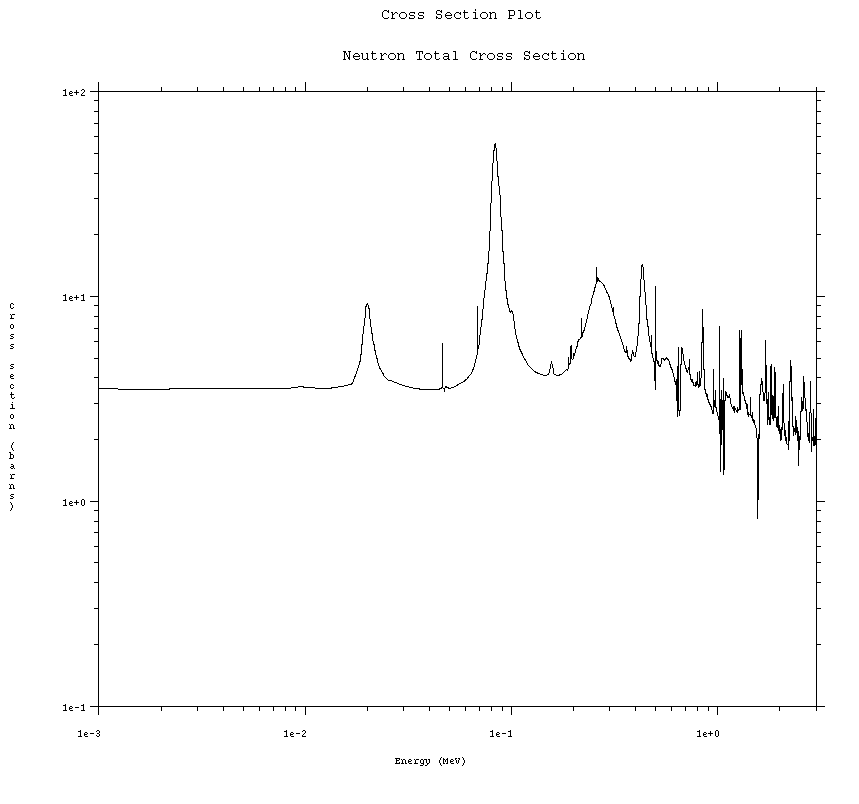
\includegraphics[width=\linewidth, height=9cm]{Master Thesis Manuel Galdon/figures/Build-up effect/cross section of Mg.png} 
    \caption{MCNP plot of the cross section in $barns$ of Mg.}
    \label{fig:Cross section of Mg}
\end{minipage}
\end{figure}

MCNP gives out the plots of the cross section of a material always in logarithmic scale. In this case, there is a sudden increase in the cross section for the energy of 0.25 \unit{\mega\electronvolt} and, for that value of the energy, the cross section is higher than for the case of 2.5 \unit{\mega\electronvolt}, which causes the plot in MCNP to show the energy deposition lines switched. 


